%%%%%%%%%%%%%%%%%%%%%%%%%%%%%%%%%%%%%%%%%%%%%%%%%%%%%%%%%%%
% --------------------------------------------------------
%  ____  _           
% |  _ \| |__   ___  
% | |_) | '_ \ / _ \ 
% |  _ <| | | | (_) |
% |_| \_\_| |_|\___/ 
%
% LaTeX2e Template
% Version 3.0.0 (24/02/2026)
%
% Author: 
% Guillermo Jimenez (memo.notess1@gmail.com)
% 
% Contributor:
% Eduardo Gracidas (eduardo.gracidas29@gmail.com)
%
% License:
% Creative Commons CC BY 4.0
% --------------------------------------------------------
%%%%%%%%%%%%%%%%%%%%%%%%%%%%%%%%%%%%%%%%%%%%%%%%%%%%%%%%%%%
% --------------------------------------------------------
% Find the latest version on GitHub:
% https://github.com/MemoJimenez/Rho-class
% --------------------------------------------------------
%%%%%%%%%%%%%%%%%%%%%%%%%%%%%%%%%%%%%%%%%%%%%%%%%%%%%%%%%%%

\documentclass[11pt,a4paper,twocolumn,twoside]{rho-class/rho}
\usepackage[spanish,es-notilde]{babel}

%% Spanish babel recomendation
% \usepackage[spanish,es-nodecimaldot,es-noindentfirst]{babel}

%----------------------------------------------------------
% Title
%----------------------------------------------------------
\doctype{Reporte de Proyecto - Ciencia de Datos para Sensores Inteligentes}
\title{Medición de consistencia en 
suelta en tiro de arco y comparacion de tecnicas de clustering}

%----------------------------------------------------------
% Authors, Affiliations and dates
%----------------------------------------------------------

\author[a]{Diana Minerva Jaramillo Durazo}


%----------------------------------------------------------

\affil[a]{Centro de Investigación Científica y de Educación Superior de Ensenada, Baja California, México.}

%----------------------------------------------------------

\dates{Abril 2026}

%----------------------------------------------------------

\docinfo{Reporte de resultados del proyecto de la materia Ciencia de Datos para Sensores Inteligentes. Proyecto relacionado con la medición de consistencia en suelta en tiro con arco utilizando sensores inerciales y métodos de clustering para analizar los datos obtenidos.} 

%----------------------------------------------------------

\theday{\today}

%----------------------------------------------------------
% Abstract and Keywords
%----------------------------------------------------------

\begin{abstract}
    Este proyecto se enfoca en la medición de los tiros que se realizan en tiro con arco, utilizando sensores inerciales para obtener datos sobre la suelta del arco. El objetivo principal es analizar la consistencia de los tiros mediante técnicas de clustering, lo que permitirá identificar patrones y variaciones en cada sujeto. Los resultados con el como se comparan 3 métodos de clustering diferentes, y se discuten las implicaciones de estos resultados para mejorar el análisis de esta área de estudio.
\end{abstract}

%----------------------------------------------------------

\keywords{Clustering, Arquería, Sensores inerciales, Consistencia, Tiro con arco.}

%----------------------------------------------------------

\begin{document}

    \maketitle
    \thispagestyle{firststyle}

%----------------------------------------------------------

\section{Introducción}

    \rhostart{E}n el ámbito del tiro con arco se tienen 5 etapas para realizar un tiro, la primera es la postura, donde el arquero se posiciona de manera correcta para realizar el tiro, la segunda es el anclaje, donde el arquero lleva la cuerda a un punto de referencia en su cara, la tercera es apuntar, donde el arquero apunta al objetivo, la cuarta es la suelta, donde el arquero libera la cuerda para que la flecha vuele hacia el objetivo, y la quinta es el seguimiento, donde el arquero mantiene su postura y observa el vuelo de la flecha. \cite{archerystages}
	
    Durante lecciones de arquería se suele hacer enfasis en que la suelta es una de las etapas mas importantes, ya que es el momento en el que se libera la cuerda y se determina la dirección y velocidad de la flecha. Se busca que el arquero pueda realizar una suelta consistente, lo que significa que cada vez que suelta la cuerda, lo hace de la misma manera, con el mismo movimiento y fuerza. Esto es importante porque una suelta inconsistente puede llevar a tiros imprecisos y resultados impredecibles y se teoriza que un movimiento severo en la suelta puede afectar la precisión del tiro. \cite{tahaCorrelationArchersHands2016c}


    \subsection{Estudios Previos}

        En la busqueda de estudios relacionados con esta area se encontraron dos que se enfocan en la medicion de los tiros en arqueria y el movimiento de la mano "Citar a zahari", en donde se concluye que el movimiento de la mano del arco y un score calculado con su aceleracion estan correlacionados al analizar el promedio maximo de desplazamiento de la amplitud de la señal al momento de la suelta. Estudio que fue realizado con arqueros de universidades que estan en nivel de competencias.
        Otro estudio realizado por Cheng-Hao Quan \cite{quanAnalysisShootingConsistency2017b}, se enfoca en la consistencia de los tiros usando un algoritmo diseñado para medir la similitud de dos secuencias de tiempo, el Dynamic Time Warping (DTW), y se concluye que entre menor sea la distancia de dos secuencias mejores eran los resultados realizados por el arquero, la variable que consideraron para el análisis fue la aceleración de un sensor colocado en el antebrazo que sostiene el arco.

\section{Metodologia}

    \subsection{Instrumentos de Medición}

        Para la medición de los tiros se utilizaron sensores inerciales, LPMS-B2, los cuales se conectaban a través de Bluetooth a una computadora para registrar los datos obtenidos. Se tuvieron problemas con los sensores, ya que se desconectaban constantemente, lo que llevó a la pérdida de datos y a la necesidad de repetir las mediciones varias veces para obtener un conjunto de datos completo.

        \figref{fig:sensor} Sensor LPMS-B2 utilizado 
    		
    \begin{figure}[H]
    	\centering
    	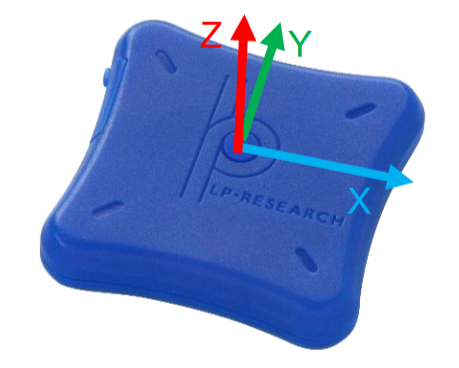
\includegraphics[width=0.7\columnwidth]{figures/sensor.PNG}
    	\caption{Ejemplo del sensor LPMS-B2 utilizado en el estudio.}
    	\label{fig:sensor}
    \end{figure}

        También se redujo la cantidad los parámetros que se median con los sensores a solo aceleración, datos del giroscopio y la aceleración lineal, ya que se consideró que estos eran los más relevantes para el análisis de la suelta en tiro con arco.
        Estos sensores se coloraron en 3 puntos clave:
        \begin{itemize}
            \item En la \emph{mano que sostiene el arco}, para medir el movimiento del arco.
            \item En la \emph{parte superior del brazo que sostiene la cuerda}, para medir el movimiento de todo el brazo que realiza la suelta.
            \item En la \emph{mano de la suelta}, para medir exactamente el punto más cercano a la suelta.
        \end{itemize}

        \figref{fig:place} Ejemplo de como quedaron colocados los sensores en el cuerpo de los sujetos evaluados
    		
    \begin{figure}[H]
    	\centering
    	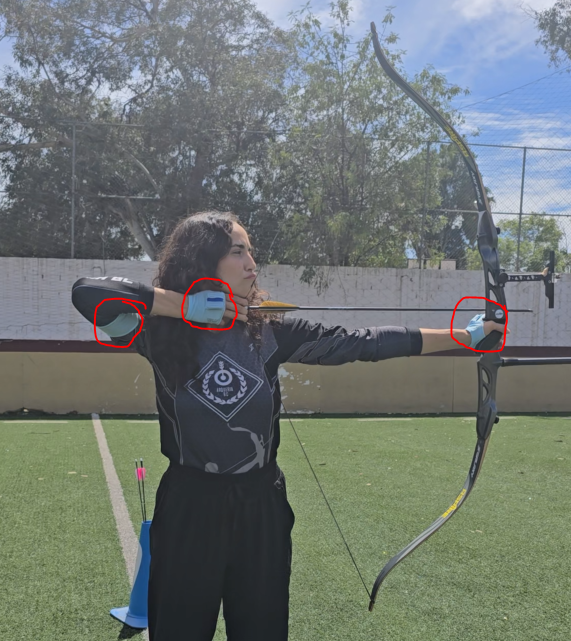
\includegraphics[width=0.7\columnwidth]{figures/colocacion.PNG}
    	\caption{Demostracion de colocacion de los sensores dentro de los circulos rojos y como se ven al momento de realizar un tiro.}
    	\label{fig:place}
    \end{figure}

        

    \subsection{Recopilación de los datos}

        Se realizaron las mediciones de los tiros con la ayuda de un grupo de arqueria local, ArqueriaBC, en las instalaciones del Colegio de Bachilleres de Baja California, plantel Ensenada. Los tiros se realizaron al aire libre y la distancia de los sujetos evaluados era la que practican normalmente, por lo que la distancia entre sujetos variaba en un rango de 26 a 30 metros.

        El total de participantes fue de 6 sujetos, con diferentes niveles de experiencia en tiro con arco, desde principiantes hasta arqueros más avanzados. Entre los participantes se incluyo a un arquero zurdo y personas sin experiencia en este deporte, para obtener una variedad de datos.

        Cada sujeto realizo 5 mediciones en las cuales se les pidio realizar 5 tiros cada una, lo que aproximaba a un total de 150 tiros en en caso de que no hubiera problemas con los sensores.

        Para recopilar los datos se hicieron unos soportes de tela transpirable y elastica para que el sensor se mantuviera fijo en su lugar durante la medición, y se les pidió a los sujetos que realizaran sus tiros de manera normal utilizando estos soportes junto con el sensor.

        Aparte se realizo un programa con Python con la libreria de OpenZen, la cual es compatible con los sensores LPMS-B2, para facilitar la recopilación de los datos y su posterior análisis. Este programa se encargaba de conectarse a los sensores, iniciar la grabación de los datos y guardarlos en un formato adecuado para su análisis posterior. Esto ya que el programa que proporciona el fabricante de los sensores no es muy exacto para la recopilación de datos, y se perdían muchos tiros debido a desconexiones o problemas técnicos.

        En este programa se implemento una función para detectar el momento de la suelta, lo que permitió segmentar los datos de cada tiro y enfocarse específicamente en el análisis de la suelta, que es el objetivo principal de este proyecto. Lo cual ayudo a separar mejor los datos y ahorrar trabajo a la hora de analizar los datos. Asi como agregar el id de lo sensores para tener control de los datos y de donde se estaban obteniendo, lo que ayudo a identificar los datos de cada sensor y su ubicación en el cuerpo del sujeto.

        Los datos se generaban a una tasa de muestreo de 200 Hz, lo que proporcionaba una resolución temporal adecuada para capturar los movimientos rápidos asociados con la suelta en tiro con arco.


    \subsection{Procesamiento de los datos}

        Los datos se procesaron en Python en un entorno de Jupyter Notebook, utilizando bibliotecas como NumPy y Pandas para la manipulación de los datos, y Matplotlib para la visualización.

        Considerando la literatura se decidió utilizar el algoritmo de Dynamic Time Warping (DTW) para medir la similitud entre las secuencias de datos obtenidas de los sensores durante la suelta. Este algoritmo es especialmente útil para comparar secuencias de tiempo que pueden variar en velocidad o duración, lo que es común en los movimientos humanos. El resultado del DTW se utilizó como un feature para evaluar la consistencia de los tiros, con la hipótesis de que tiros más consistentes tendrían una menor distancia DTW entre ellos.

        Para filtrar los datos y eliminar el ruido, se utilizó el filtro de Savitzky-Golay, el cual se seleccionó por su característica de eliminar el ruido mientras preserva las características importantes de la señal, como los picos y las formas de onda. Este filtro es especialmente útil para datos de sensores, donde el ruido puede ser un problema significativo. \cite{konstantinovskyIntroductionSavitzkyGolayFilter2024}

        Como parte del análisis, se aplicaron técnicas de clustering para agrupar los tiros según su similitud. Se seleccionaron tres métodos de clustering diferentes: K-means, DBSCAN y Agglomerative Clustering.
        K-means es de los metodos de clustering mas utilizados en machine learning, se puede aplicar a datos no etiquetados y es eficiente para grandes conjuntos de datos. \cite{winlandQueEsAgrupacion2024} DBSCAN es un método de clustering que funciona detectando areas de concentración de puntos, lo que lo hace útil para detectar clusters de forma arbitraria, en caso de que los puntos no sean parte de los clusters se consideran ruido. \cite{birantSTDBSCANAlgorithmClustering2007} Agglomerative Clustering es un método de clustering jerárquico que construye un árbol de clusters, comenzando con cada punto como un cluster individual y fusionándolos iterativamente según su similitud. \cite{AgglomerativeClustering}

        Cada uno de estos métodos tiene sus propias características y ventajas, lo que permitió comparar los resultados obtenidos con cada uno y evaluar cuál era más efectivo para este tipo de datos y ver como se agrupaban los tiros según los features que se seleccionaron.

\section{Resultados}

    En el análisis exploratorio de los datos se observó que hubo una gran cantidad de tiros perdidos debido a problemas con los sensores, lo que redujo significativamente el tamaño del conjunto de datos disponible para el análisis. Sin embargo, se logró obtener un conjunto de datos suficiente para realizar un análisis preliminar.

    La cantidad de tiros que fueron analizados por persona fueron de 21 a 25, (una perdida de 0 a 4 tiros) lo cual es una cantidad algo limitada para realizar un análisis estadístico robusto, pero se pueden obtener algunas conclusiones preliminares sobre la consistencia de los tiros y la efectividad de los métodos de clustering seleccionados.

    Se seleccionaron dos conjuntos distintos de features para el análisis de clustering. El primer conjunto incluyó la distancia DTW entre los features de Pitch\_Angle (deg), Roll\_Angle (deg), AccZ (g)\_sg, LinAccX (g), LinAccY (g), LinAccZ (g), los cuales se consideraban relevantes para este análisis. El segundo conjunto de features se centró únicamente en la distancia DTW entre los features de Pitch\_Angle (deg), Roll\_Angle (deg) y AccZ (g)\_sg, con la hipótesis de que estos podrían ser los más directamente relacionados con la consistencia de la suelta y al ser menos features se compararia si es mejor para el análisis de clustering.

    Al realizar el análisis de clustering con ambos conjuntos de features, se observó que los resultados variaban según el método de clustering utilizado. En general, se encontró que K-means tendía a agrupar los tiros de manera más clara, mientras que DBSCAN y Agglomerative Clustering mostraban una mayor dispersión en los clusters formados. 

    Al calcular el silhouette score para evaluar la calidad de los clusters formados, se obtuvieron los resultados que se muestran en la tabla \ref{tab:results}. En general, el método de clustering que obtuvo el mejor silhouette score variaba dependiendo de cada sujeto y el conjunto de features utilizado.

    \tabref{tab:results} Resultados de Silhouette Score promedio para cada método de clustering y conjunto de features. 
    \begin{table}[H]
        	\caption{Promedio de Silhouette Score para cada método de clustering y conjunto de features.}
        	\label{tab:results}
        	\begin{tabular}{
        		>{\raggedright\arraybackslash}p{0.25\columnwidth}
        		>{\raggedright\arraybackslash}p{0.29\columnwidth}
        		>{\raggedright\arraybackslash}p{0.31\columnwidth}
        	}
        	\toprule
        	\textbf{Metodo de clustering} & \textbf{Todos los features seleccionados} & \textbf{Menos features} \\
        	\midrule
        	Agglomerative & 0.322 & 0.304 \\
        	DBSCAN & 0.163 & 0.169 \\
        	K-Means & 0.250 & 0.276 \\
        	\bottomrule
        	\end{tabular}
            \tabletext{Nota: El valor maximo que se obtuvo fue de 0.60 para el sujeto 4 con el metodo de clustering K-means y el metodo agglomerative, este resultado lo dio con ambos sets de features.}
        \end{table}
        

\section{Graficas de los Datos y Visualizaciones}
		
    \figref{fig:figure} Muestra de datos crudos de un sensor durante una sesion de tiro
    		
    \begin{figure}[H]
    	\centering
    	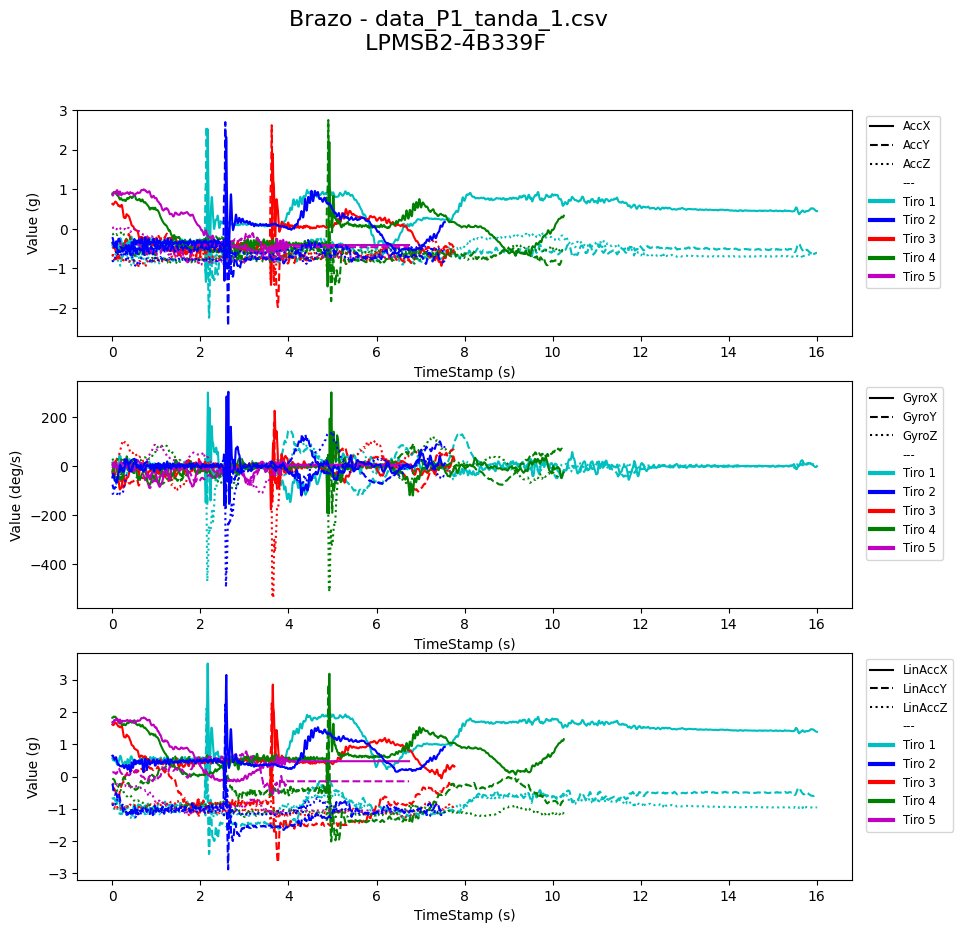
\includegraphics[width=0.7\columnwidth]{figures/datosrawsensor.png}
    	\caption{Datos crudos de un sensor durante una sesión de tiro. En esta gráfica se pueden observar las diferentes señales obtenidas por el sensor, como la aceleración, datos del giroscopio y datos de aceleración lineal, lo que proporciona información sobre el movimiento del arquero durante la suelta.}
    	\label{fig:figure}
    \end{figure}

    \figref{fig:figure2} Muestra de datos filtrados de un sensor durante una sesion de tiro
    		
    \begin{figure}[H]
    	\centering
    	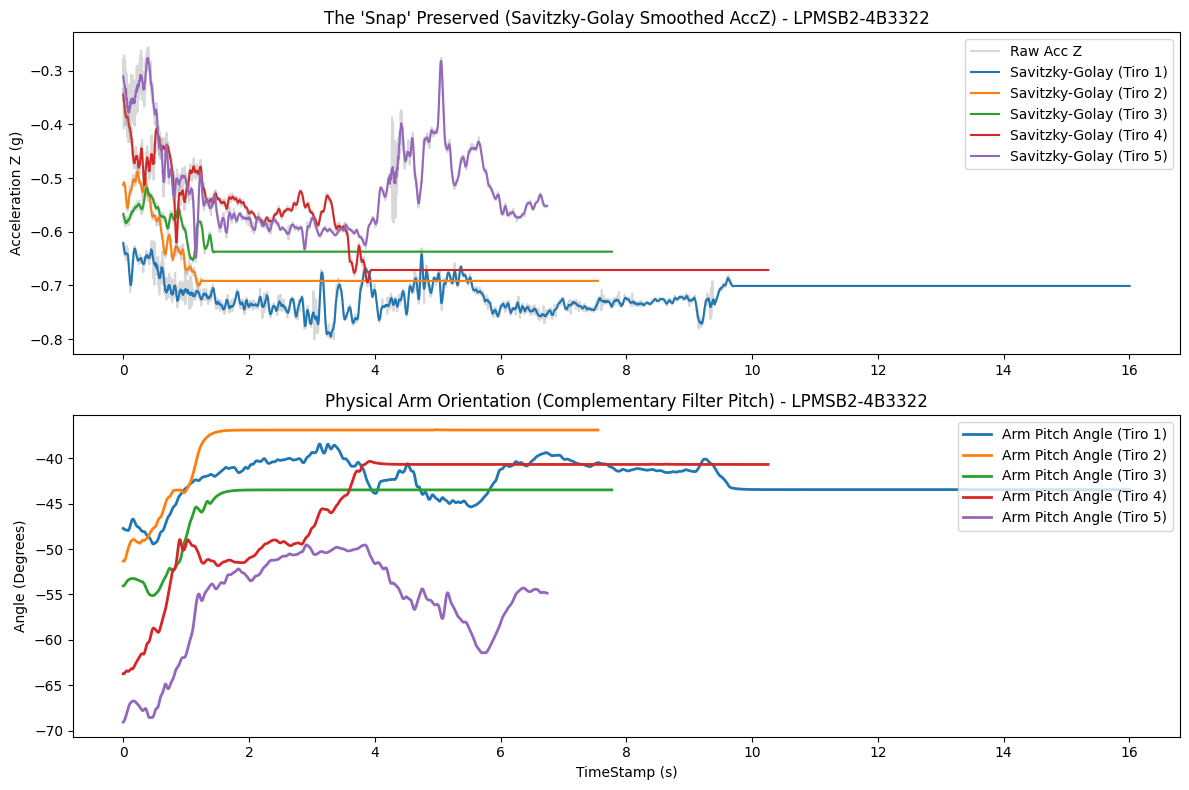
\includegraphics[width=0.7\columnwidth]{figures/filtered.png}
    	\caption{Datos de uno de los sensores después de aplicar el filtro de Savitzky-Golay. En esta gráfica se pueden observar las señales filtradas, lo que permite una mejor visualización de las características importantes de la señal, como los picos y las formas de onda, mientras se ha reducido el ruido presente en los datos crudos. Esto facilita el análisis posterior y la aplicación de técnicas de clustering para evaluar la consistencia de los tiros.}
    	\label{fig:figure2}
    \end{figure}

    \figref{fig:figure3} Análisis de como se comparan los datos usando DTW
    		
    \begin{figure}[H]
    	\centering
    	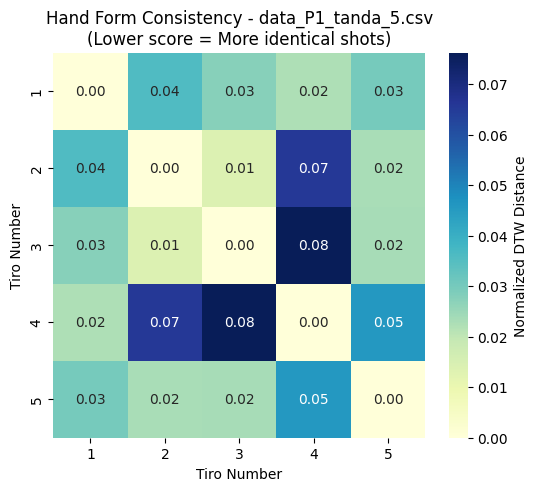
\includegraphics[width=0.7\columnwidth]{figures/dtwanalisis.png}
    	\caption{Muestra de como se comparan los tiros utilizando el algoritmo de Dynamic Time Warping (DTW). Un valor de distancia DTW más bajo indica una mayor similitud entre las secuencias de datos, lo que sugiere una mayor consistencia en la suelta. }
    	\label{fig:figure3}
    \end{figure}

    \subsection{Graficas de los Clusters finales}

    \figref{fig:full1} Metodo Aglomerative con todos los features seleccionados
    		
    \begin{figure}[H]
    	\centering
    	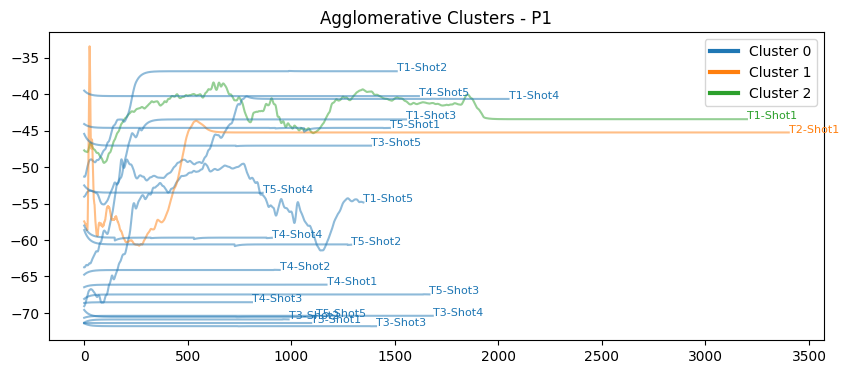
\includegraphics[width=0.7\columnwidth]{figures/clusterfull1.png}
    	\caption{Clusters formados con el metodo Agglomerative utilizando todos los features seleccionados.}
    	\label{fig:full1}
    \end{figure}

    \figref{fig:full2} Metodo DBSCAN con todos los features seleccionados
    		
    \begin{figure}[H]
    	\centering
    	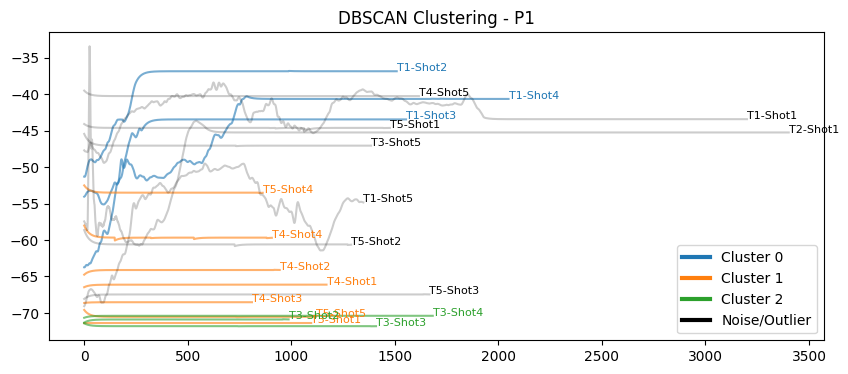
\includegraphics[width=0.7\columnwidth]{figures/clusterfull2.png}
    	\caption{Clusters formados con el metodo DBSCAN utilizando todos los features seleccionados.}
    	\label{fig:full2}
    \end{figure}

    \figref{fig:full3} Metodo K-Means con todos los features seleccionados
    		
    \begin{figure}[H]
    	\centering
    	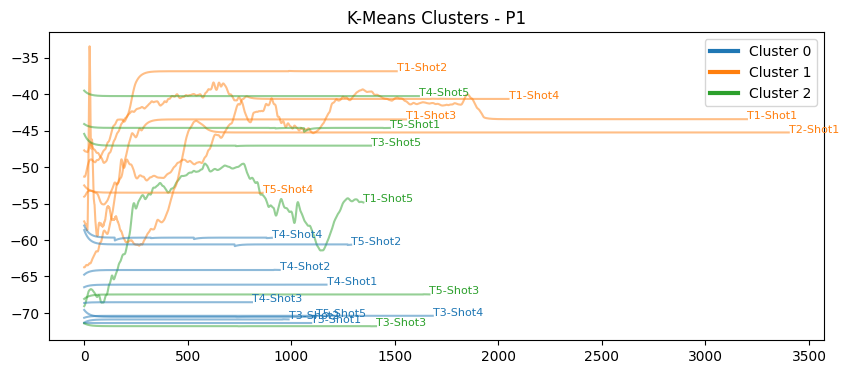
\includegraphics[width=0.7\columnwidth]{figures/clusterfull3.png}
    	\caption{Clusters formados con el metodo K-Means utilizando todos los features seleccionados.}
    	\label{fig:full3}
    \end{figure}

        \figref{fig:less1} Metodo Aglomerative con menos features seleccionados
    		
    \begin{figure}[H]
    	\centering
    	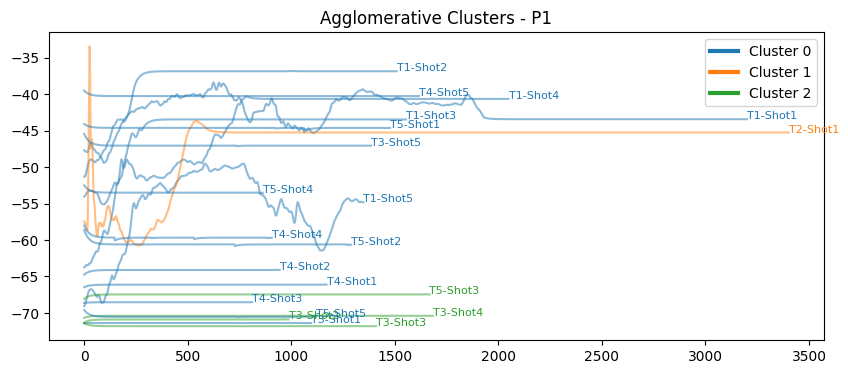
\includegraphics[width=0.7\columnwidth]{figures/clusterless1.png}
    	\caption{Clusters formados con el metodo Agglomerative utilizando menos features seleccionados.}
    	\label{fig:less1}
    \end{figure}

        
        \figref{fig:less2} Metodo DBSCAN con menos features seleccionados
    \begin{figure}[H]
    	\centering
    	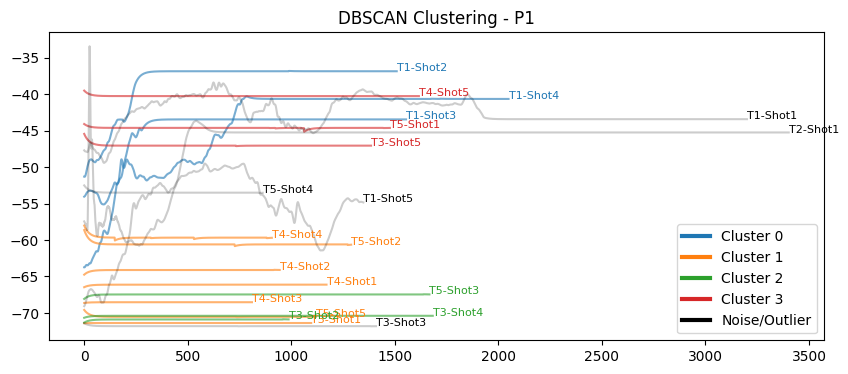
\includegraphics[width=0.7\columnwidth]{figures/clusterless2.png}
    	\caption{Clusters formados con el metodo DBSCAN utilizando menos features seleccionados.}
    	\label{fig:less2}
    \end{figure}

        
        \figref{fig:less3} Metodo K-Means con menos features seleccionados
    \begin{figure}[H]
    	\centering
    	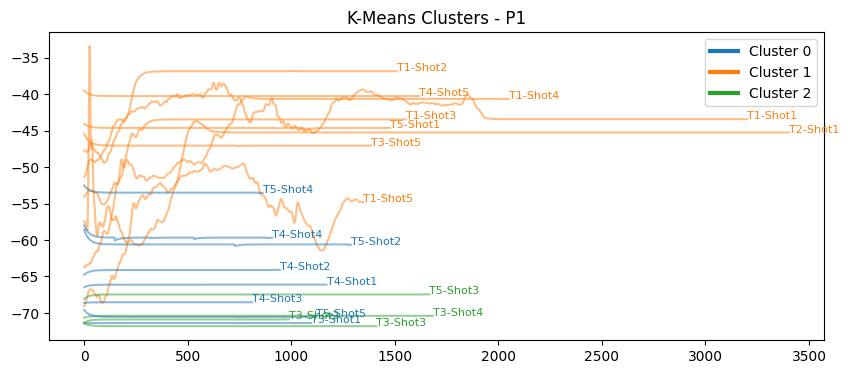
\includegraphics[width=0.7\columnwidth]{figures/clusterless3.png}
    	\caption{Clusters formados con el metodo K-Means utilizando menos features seleccionados.}
    	\label{fig:less3}
    \end{figure}


    \figref{fig:final} Comparacion en plano 2D de los clusters creados con los tres metodos de clustering utilizando todos los features seleccionados
    		
    \begin{figure}[H]
    	\centering
    	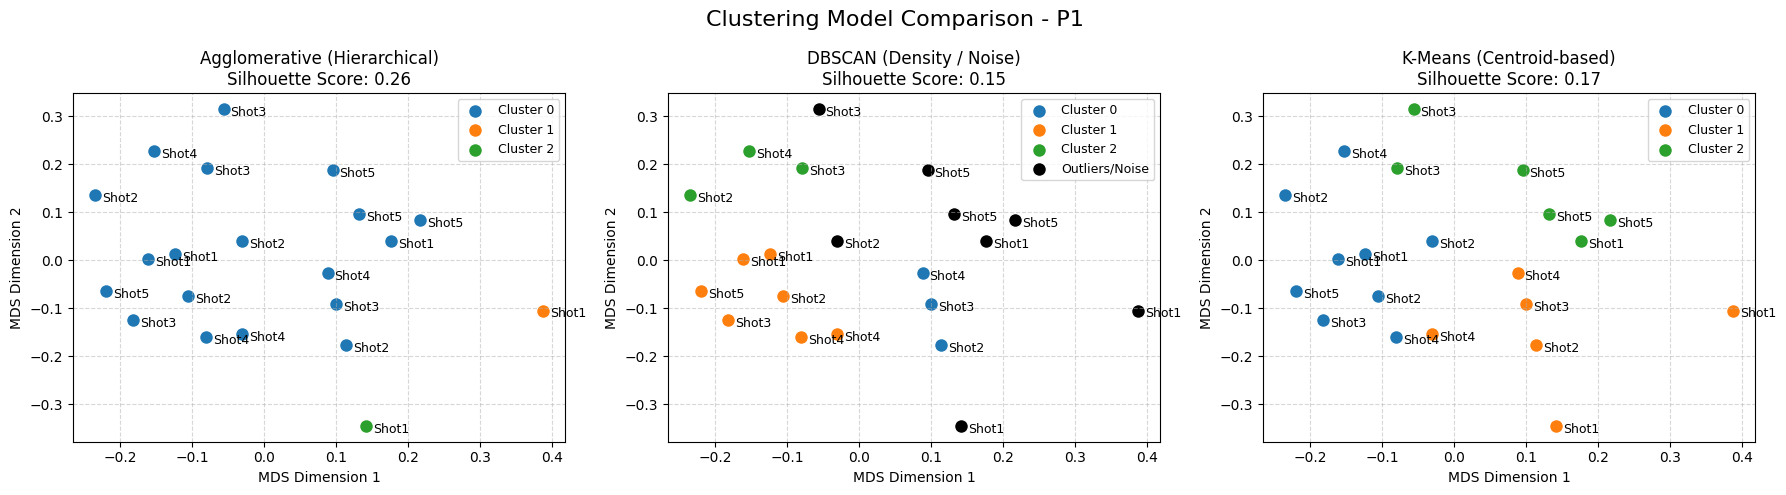
\includegraphics[width=0.7\columnwidth]{figures/comparacionfull.png}
    	\caption{Comparacion de como se verian los clusters formados con los tres metodos de clustering utilizando todos los features seleccionados en un plano 2D.}
    	\label{fig:final}
    \end{figure}

    \figref{fig:final2} Comparacion en plano 2D de los clusters creados con los tres metodos de clustering utilizando todos los features menos seleccionados
    		
    \begin{figure}[H]
    	\centering
    	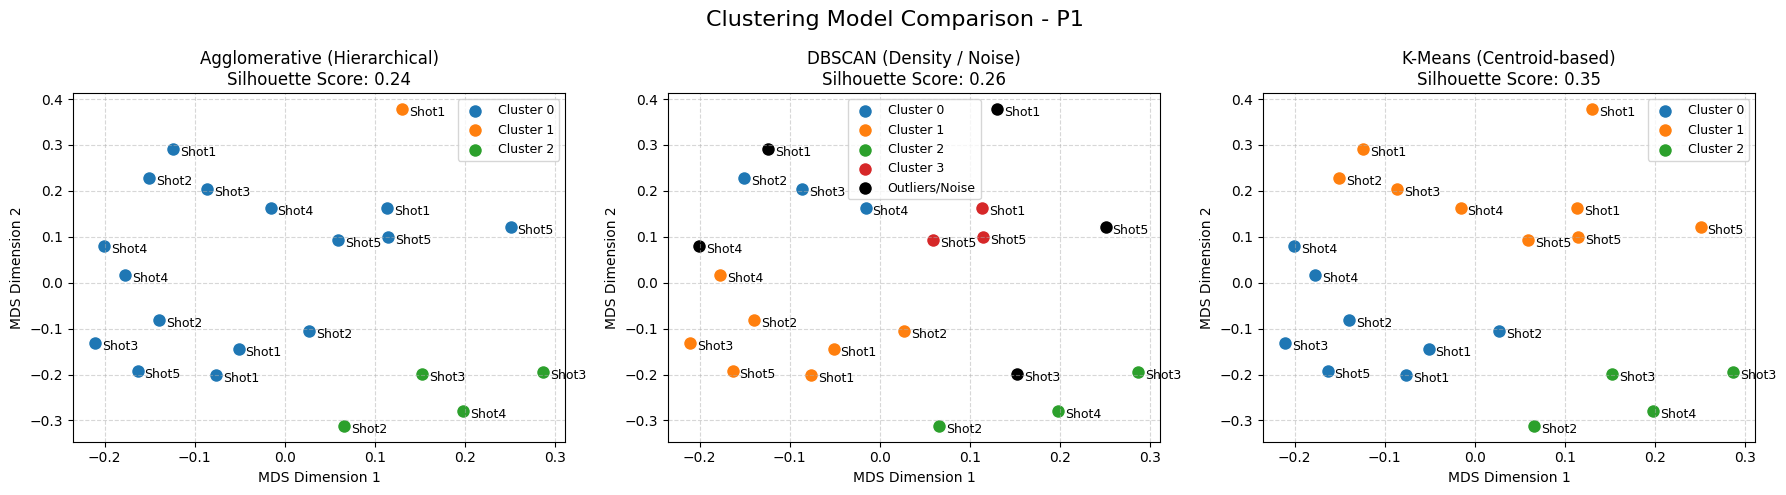
\includegraphics[width=0.7\columnwidth]{figures/compless2.png}
    	\caption{Comparacion de como se verian los clusters formados con los tres metodos de clustering utilizando todos los features menos seleccionados en un plano 2D.}
    	\label{fig:final2}
    \end{figure}


\section{Discusion}

    \subsection{Resultados obtenidos}

        En general, los resultados obtenidos muestran que el método de clustering K-means tendió a formar clusters más definidos en comparación con DBSCAN y Agglomerative Clustering. Sin embargo, la calidad de los clusters varió según el conjunto de features utilizado, lo que sugiere que la selección de features es un factor importante a considerar en este tipo de análisis.

        El hecho de que el valor máximo de silhouette score obtenido fue de 0.60 para el sujeto 4 con el método de clustering K-means y Agglomerative Clustering, sugiere que hay una cierta consistencia en los tiros de ese sujeto, aunque no es un resultado extremadamente alto. Esto podría indicar que hay variabilidad en la suelta del arquero, lo que es común en movimientos humanos.

    \subsection{Limitaciones del estudio}

        \subsubsection{Datos}

            La cantidad de datos se vio limitada al tener problemas con los sensores, el tener que buscar como lograr que los 3 sensores no se desconectaran en el momento y que no se tenga perdida de datos tomo mas tiempo de lo esperado.

        \subsubsection{Sujetos}

            El numero de sujetos evaluados fue solo de 6 al tener limitado el uso de el espacio de practica de tiro con arco, la medición de los tiros tomaba tiempo y los problemas previamente mencionanados con los sensores, lo que limitó la cantidad de sujetos que se pudieron evaluar.

\section{Conclusiones}

    En conclusión, este proyecto permitió analizar la similitud de los tiros en arqueria utilizando sensores inerciales y técnicas de clustering. A pesar de las limitaciones en la cantidad de datos y sujetos, se logró obtener información valiosa sobre la suelta en tiro con arco y cómo diferentes métodos de clustering pueden agrupar los tiros según su similitud. 

    Los resultados sugieren que el método de clustering K-means puede ser más efectivo para este tipo de análisis, aunque la selección de features también juega un papel importante. Para futuros estudios, se recomienda aumentar la cantidad de datos y sujetos evaluados, así como explorar otras técnicas de análisis y características adicionales que puedan ser relevantes para evaluar la consistencia en tiro con arco.


\section{Codigos}

	El codigo para la recopilacion de los datos y el análisis se encuentra disponible en el repositorio de GitHub asociado a este proyecto, el cual se puede acceder a través del siguiente enlace: \url{https://github.com/DianaJaramilloDurazo/CDSI-2026/tree/main/Proyecto}

\section{Bibliografia}
		
	Referencias bibliográficas utilizadas en este proyecto.


%----------------------------------------------------------

\printbibliography

%----------------------------------------------------------

\end{document}